\documentclass{mcmthesis}
\mcmsetup{CTeX = false,
        tcn = 84802, problem = B,
        sheet = true, titleinsheet = true, keywordsinsheet = true,
        titlepage = true, abstract = true}
\usepackage{palatino}
\usepackage{lipsum}
\usepackage{verbatim}


\title{Prediction of languange distribution}

\date{\today}
\begin{document}
\begin{abstract}
\qquad This paper is about to propose a predictable model which is forecasting the number of each native speaker and total speark in the next 50 years.
Also, the model would be used to commercial field, it could find a better place to open a office which can make huge benefit towards a service company.
And at last, due to the changing nature of global communcation, in order to save the resources of the company, we calculate the profits that the company earn and losses.
The results is to suggest the company whether open six office or not.


We first model the trend of number of native speaker based Fuzzy Synthetic Evaluation Model, forecast the change of distribution.

Secondly, we simulate the trend of migration by using Markov Chain Model. 

Thirdly, we test the model by using his torical data, we give the criterion that percentage difference should be under 5\%
As well as we note that the model's strength and weaknesses, which can only refer limited years and the model's creditability would decrease as the time through.

·
Finally, the model would be detected using the real results.

\begin{keywords}
Population; Native speaker ; Fuzzy Synthetic Evaluation Model : Markov Chain Model
\end{keywords}
\end{abstract}
\maketitle
\tableofcontents
\section{Introduction}
\subsection{Background}
\qquad Nowadays,There are 7099 languages around the world. Each of the language has its unique charm.
But they are spread unequally throughout the world. 
That trend is clear whether we’re looking at whole regions,or individual countries.
Under the influence of globalization,the distribution and number of each language speaker are now very different from the past. 
It is changing all the time.
\cite{No-of-languages}


Moreover,an increasing number of people who learn another languages as second language even third languange or above. 
Some may know English, Chinese, Spanish and some may know Japanese, Portuguese. These kind of people who require the language job in service company.
The head hunter had noticed that the phenomenon. 

So we established this model to predict the distribution of the languages in the next 50 years. A further data can improve the business by decreasing
the probability of mistakes to open a office. The place would be considered and selected depand on economic index from the model.
It could be easy to refer which language would become popular in the corresponding place in the future. Besides,
it would be offering the job opportunity directly to someone in need who satisfied the language requirement.Turning job finding to be more convenient.
On the other hand, considering the people in these places who can speak more then on language, and they are the 
main targets to employ. The distribution of number of languages used can be review.
 
 
According to the study \cite{hel},\emph{"For a company entering a new market, language can be a major barrier that firms
may underestimate(Freeman and Sandwell 2008),and understanding language influence across different markets is important for international companies.)" }
The sentence above shows the relation between economic development and languange distribution. As we know, the quality of the service demands variety of the languages in the world.
The country which attract more tourist visiting , the more understanding and acceptable of foreign language. 
That's how the top service company can earn more profits from others.



The total number of speaker is mainly affected by the population growth. The following graph shows the relationship between number of speaker and the population


We focus exclusively on the second definition.

\subsection{Assumptions}
\qquad The model is going to ignore unpredictable and high-impact occured, we have to make following assumptions to guarantee the correctness of the model.
\begin{itemize}
\item ensure the information is absolutely right, 
\item the governments won't change the official language in their country,
\item ignore the large-scale war, assume it won't break,
\item assume the corporate taxes won't change,

\end{itemize}


\begin{Theorem} \label{thm:latex}
\begin{equation}\int^x_\infty x \mathrm{d}F_\iota(x)
\end{equation}
\end{Theorem}

\section{Analysis of the Problem}
\subsection{Overall analysis}

The trend of the emigration reviews the trend of language distribution in the next 50 years.

\subsection{Key point analysis}
\subsubsection{Analysis of prediction of native speaker growth}

\subsubsection{Analysis of prediction of the emigration percentage between countries}
\qquad The second prdiction is based on the data of Emigration, and we set the model that country to country, and use the percentage of the emigration to 
form a probability model.According to a study\cite{tec} \emph{"It is a quantitative description of the application of Markov
mode on the migration"} We note that the trend of emigration is avalible to apply for Markov Chain Model.  
The emmigration should satisfy the Markov Chain conditions which is trend only depand on the next data but not earlier.

\section{The models}
\subsection{Notations}
We will use the symbols that given in the following table.
\begin{table}[h]
\begin{center}
\begin{tabular}{c l}
\hline
\multicolumn{1}{l}{Variable} & Description                                      \\
\hline
$L_i$                            & Number of first(second,third or above) language (i=1 for first,etc)                                       \\
$ Eg_i  $                         &Number of Emigration of country i                                      \\
$ Ig_i  $                     &Number of Immigration of country i\\
$\ell_{ij}   $                       &The percentage of emigration from Country i to Country j                                         \\
P                            & Population                                \\
$P_{GDP}   $                         & Per Capita GDP                                   \\
Im                            & Import (dollar)                                       \\
Ex                            & Export (dollar)                                   \\
\hline
\end{tabular}
\end{center}
\end{table}

\subsection{The model idea}
\qquad Due to the lack of data for the number of native speaker, we consider the Fuzzy Synthetic Evaluation Model to simulate the growth of speakers in the next 50 years.
As we have found the factor of native speaker's growth has a strong relation with population growth of the countries which take it as official language.

\subsection{Fuzzy Synthetic Evaluation Model}

\qquad We construct this model because it's a command evaluation method to reserve the mainly influence factor. Which affect the countries influences in the future. The factor can be divided at three part in this problem,
native speaker, economy and social culture. Those factors are difficule defined as actual value directly. So as to evaluate, we have secondary indicator, 
using second-level fuzzy syntheic evaluation model. We divide each factors in futher detail. The table will be listed in the followiing:
\begin{table}[h]
\begin{center}
\hspace{-1in}

\fontsize{10}{12}\selectfont
\setlength{\tabcolsep}{10mm} 
\begin{tabular}{l l}
\toprule
\textbf{Primary indicator}     & \textbf{Secondary indicator}    \\
\midrule
\addlinespace

Native speaker & Number of native speakers  \\
\addlinespace
\multirow{2}{*}{Economy}    & GDP(Gross domestic product) \\
 &FDI(Foreign Direct Investment)\\
\addlinespace

\multirow{3}{*}{Social culture} &  Number of official language school \\
 &Immigration \\
 &Language on internet \\

\bottomrule
\end{tabular}

\caption{System of language development indicator of each country's influences}
\end{center}
\end{table}
\\
 \qquad As we have constructed a model, there are 3 step to us to quantify the data shown above.

\paragraph {Step 1:} Define the weight of each indicator that associate the influences of a language

\paragraph {Step 2:} 

\paragraph {Step 3:}asd

\eqref{aa}

\begin{equation}
a^2 \label{aa}
\end{equation}

\[
  p_{j}=\begin{cases} 0,&\text{if $j$ is odd}\\
  r!\,(-1)^{j/2},&\text{if $j$ is even}
  \end{cases}
\]



\[
  \arcsin \theta  =
  \mathop{{\int\!\!\!\!\!\int\!\!\!\!\!\int}\mkern-31.2mu
  \bigodot}\limits_\varphi
  {\mathop {\lim }\limits_{x \to \infty } \frac{{n!}}{{r!\left( {n - r}
  \right)!}}} \eqno (1)
\]
\subsubsection{The model result}

\subsection{Markov Chain Model}
Given that we have the data of population and emigration of each country, we are going to model the distribution and the trend 
of the shifting population by country.
\subsubsection{Futher assumptions}
In this model, we assumpt that the death rate are constant since there are no much data to prdict and ensure. 
\subsubsection{Modelling}
We can have the following model based on the data on 2017\\

\begin{displaymath}
Let \quad T=
  \begin{pmatrix}
  {\ell_{11} } & {\ell_{12} } & \cdots &{\ell_{1n} }  \\
  {\ell_{21} } & {\ell_{22} } & \cdots & {\ell_{2n} }  \\
  {\vdots } &  {\vdots }  & \ddots &   \vdots \\
  {\ell_{11} } & {\ell_{12} } & \cdots &{\ell_{nn} }  \\
  \end{pmatrix}
  \qquad \sum^n_{i=1}=\ell_{ij}=1 \qquad (j=1,2,\cdots,n)
\end{displaymath}

Matrix T refers to the distribution percentage of the emigration for each countries.
And sum of each row is 1. Considering Markove Chain Model, notice that $T^n$ is upbounded for all integer n when
the n is approaching to $\infty$, we obtain a stable Matrix P.
\begin{displaymath}
P=\lim_{n \to +\infty}T^n
\end{displaymath}
P satisfied the following conditions.
\begin{displaymath}
P=
  \begin{pmatrix}
  {p_{11} } & {p_{12} } & \cdots &{p_{1n} }  \\
  {p_{21} } & {p_{22} } & \cdots & {p_{2n} }  \\
  {\vdots } &  {\vdots }  & \ddots &   \vdots \\
  {p_{11} } & {p_{12} } & \cdots &{p_{nn} }  \\
  \end{pmatrix}
  \qquad \sum^n_{i=1}=p_{ij}=1 \qquad (j=1,2,\cdots,n)
\end{displaymath}
\qquad And P is the patterns of distribution for emigration to each countries in future.

\subsubsection{Prdiction in next 50 year}
When we get the trend above, we construct the model to descriebe the change within 50 years.
In the following,

\begin{equation}
 \text{ The set of shifting population of country i to others in one year }= (X_{i} \cdot Eg_{i})P
\end{equation}
Where $X_{i}$ and $ Eg_{i}$ refer to the set of country population and Emigration.

For forecasting the 50 years, the model construction world be like this.\\
Let $V_i$ = The set of shifting population of country i in next 50 years (each year) 
\begin{displaymath}
V=\begin{pmatrix}
  {V_{1} }  \\
  {V_{2} }  \\
  {\vdots } \\
  {V_{n} }  \\
  \end{pmatrix}
\qquad  \text {n for the number of country}
\end{displaymath}

\begin{equation}
V_i = \{(X_{i1} \cdot Eg_{i})P, (X_{i2} \cdot Eg_{i2})P^2, \cdots, (X_{i 50} \cdot Eg_{i 50})P^{50}\}
\end{equation}
And we obtain the actual prediction on the distribution of emigration in next 50 year (each year).
As for the immigration, 
we let $P'=P $(P'is the transpose of P), P’ reviews the percentage distribution of the country which from others.we can take the same action to establish the model.
We let the following Q for infinity of T', the reason is the same to the construction of P:
\begin{displaymath}
Q=\lim_{n \to \infty} T'
\end{displaymath}
After taking the limitation, total coming population of country i in one year can be written as $U_i$ vector form such as before we made.
\begin{displaymath}
U=\begin{pmatrix}
  {U_{1} }  \\
  {U_{2} }  \\
  {\vdots } \\
  {U_{n} }  \\
  \end{pmatrix}
\end{displaymath}
By using the data of immigration of each country form each country, we can write down the following equation.

\begin{equation}
U_i = \{(X_{i1} \cdot Ig_{i})Q, (X_{i2} \cdot Ig_{i2})Q^2, \cdots, (U_{i 50} \cdot Ig_{i 50})Q^{50}\}
\end{equation}

After finishing the model, we obtain Matrix V and U , which is direcely indicate the flow of distribution of language in next 50 years.

\subsection{Filtering Model for choosing the place }
This model will be divieded at three filtering for the best 6 countries to open the office, 
\subsubsection {First filtering}

\subsubsection {Second filtering}

\subsubsection {Third filtering}

A good place for service company should consider the environmen, economy and policy towards investment.Refer to the essay \cite{eiu}, using the indicator 
from questionnatire to evaluate whether the place is good for business or not. We construct the similar model by using a few data from the resources.
The indicators of business place will be listed in the following:
\begin{itemize}
\item \textbf{GDP}\\
GDP is one of most important factor that we consider, it affects the short term development of a country, which is a business index around the world.
\item \textbf{Corporation taxes}\\
Balancing the cost spend on taxex and the benefit, the problem that company should consider.
\item \textbf{GDP's growth} \\
GDP's growth indicates the long term development of a country, business affairs will be affected in the future.
\end{itemize}
These are the main factors influence the company's prospect. Our model are based on these three indicators to evaluate. 

\section{Calculating and Simplifying the Model }
\qquad We analysis how the factors affecting the influences of a countries,
using the data from \cite{a}, we had let the weight of each factor in the 
evaluation model shown in the following.
\begin{table}[h]
\begin{center}
{\hspace{-1in}

\fontsize{10}{12}\selectfont
\begin{minipage}{\textwidth}
\begin{tabular}[c]{c c c c}
\toprule
\multirow{2}{*}{Primary indicator} & Weight of primary    & \multirow{2}{*}{Secondary indicator} &  Weight of secondary       \\
 & indicator & & indicator \\
\addlinespace
\toprule
\addlinespace
Native speaker & 0.5 & Number of native speakers & 0.2 \\
\addlinespace
\hline
\addlinespace
\multirow{2}{*}{Economy}    & \multirow{2}{*}{0.3} & GDP &  0.3\\
 & & FDI & 0.2\\
\addlinespace
\hline
 \addlinespace
\multirow{3}{*}{Social culture} & \multirow{3}{*}{0.2} &  Number of official language school &  0.1\\
 & &Immigration & 0.05\\

 & &Language on internet &0.09\\
\addlinespace
\bottomrule
\end{tabular}
\end{minipage}

}\caption{The weights of each indicator}%
\end{center}
\end{table}

\begin{figure}[h]
\centering
\begin{minipage}[t]{0.48\textwidth}
\raggedright
\small
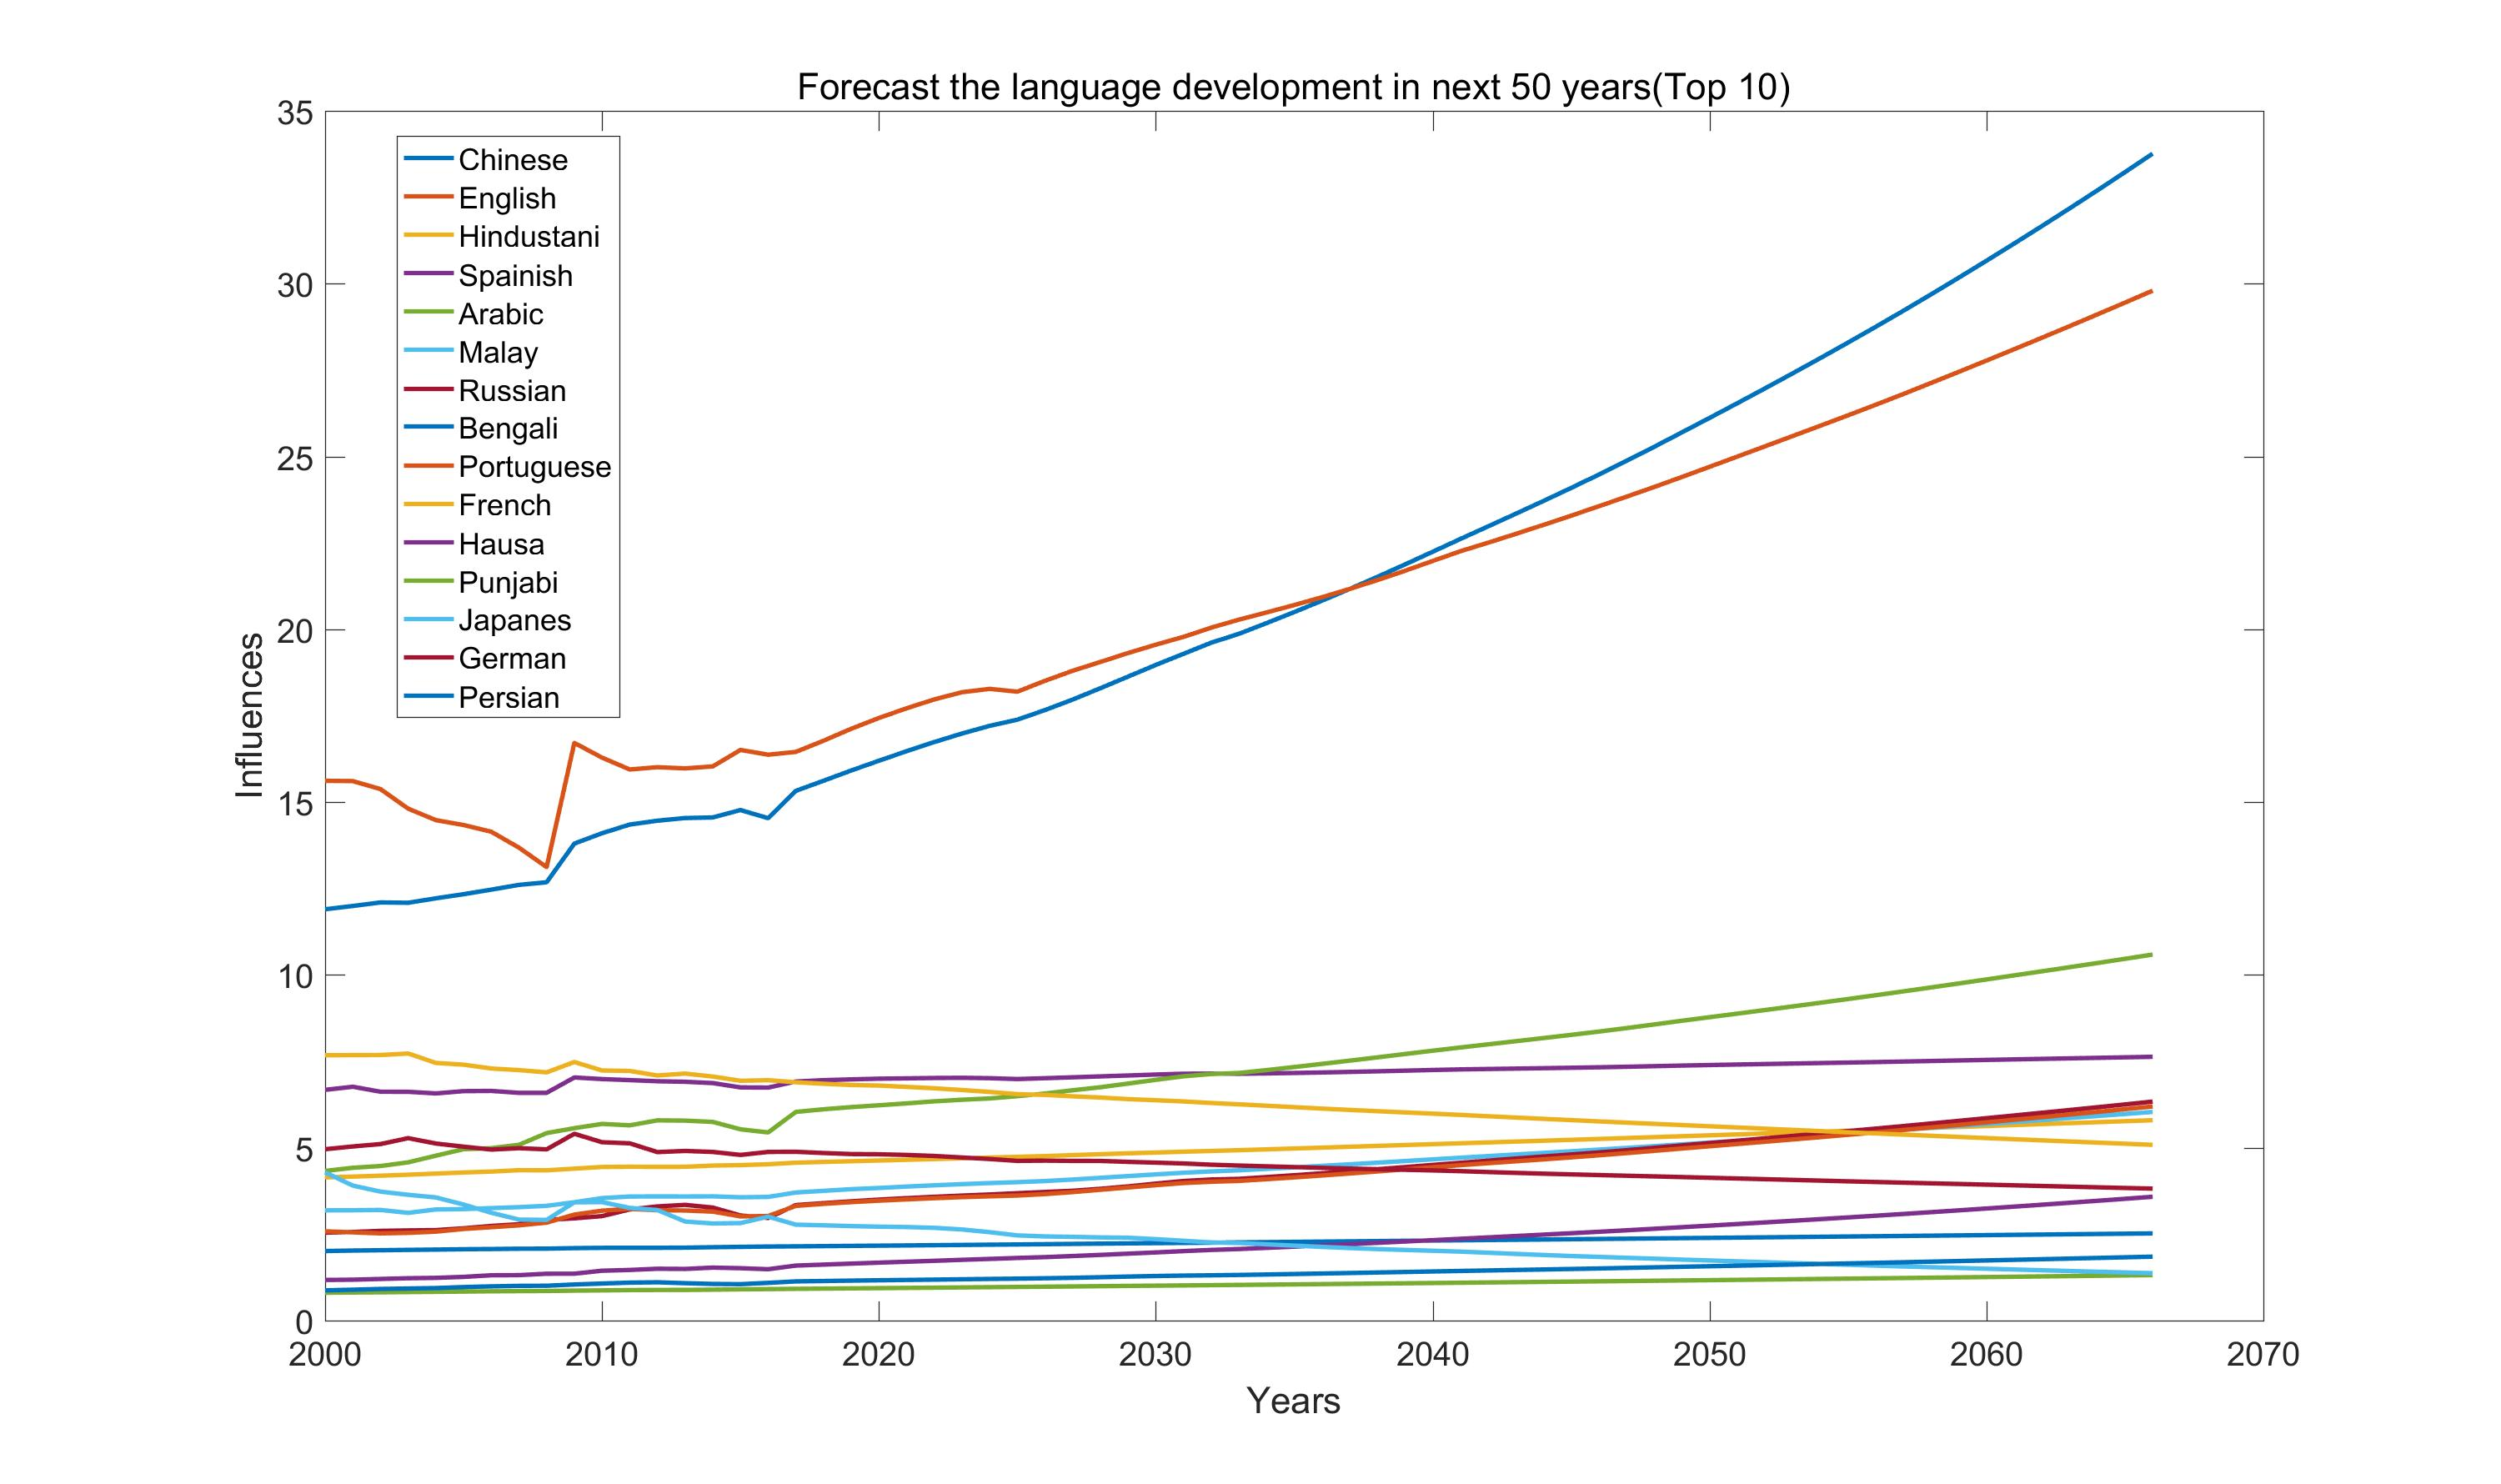
\includegraphics[width=7.5cm]{icf.jpg}
\caption{Influences ranking prediction }
\end{minipage}
\begin{minipage}[t]{0.48\textwidth}
\raggedright
\small
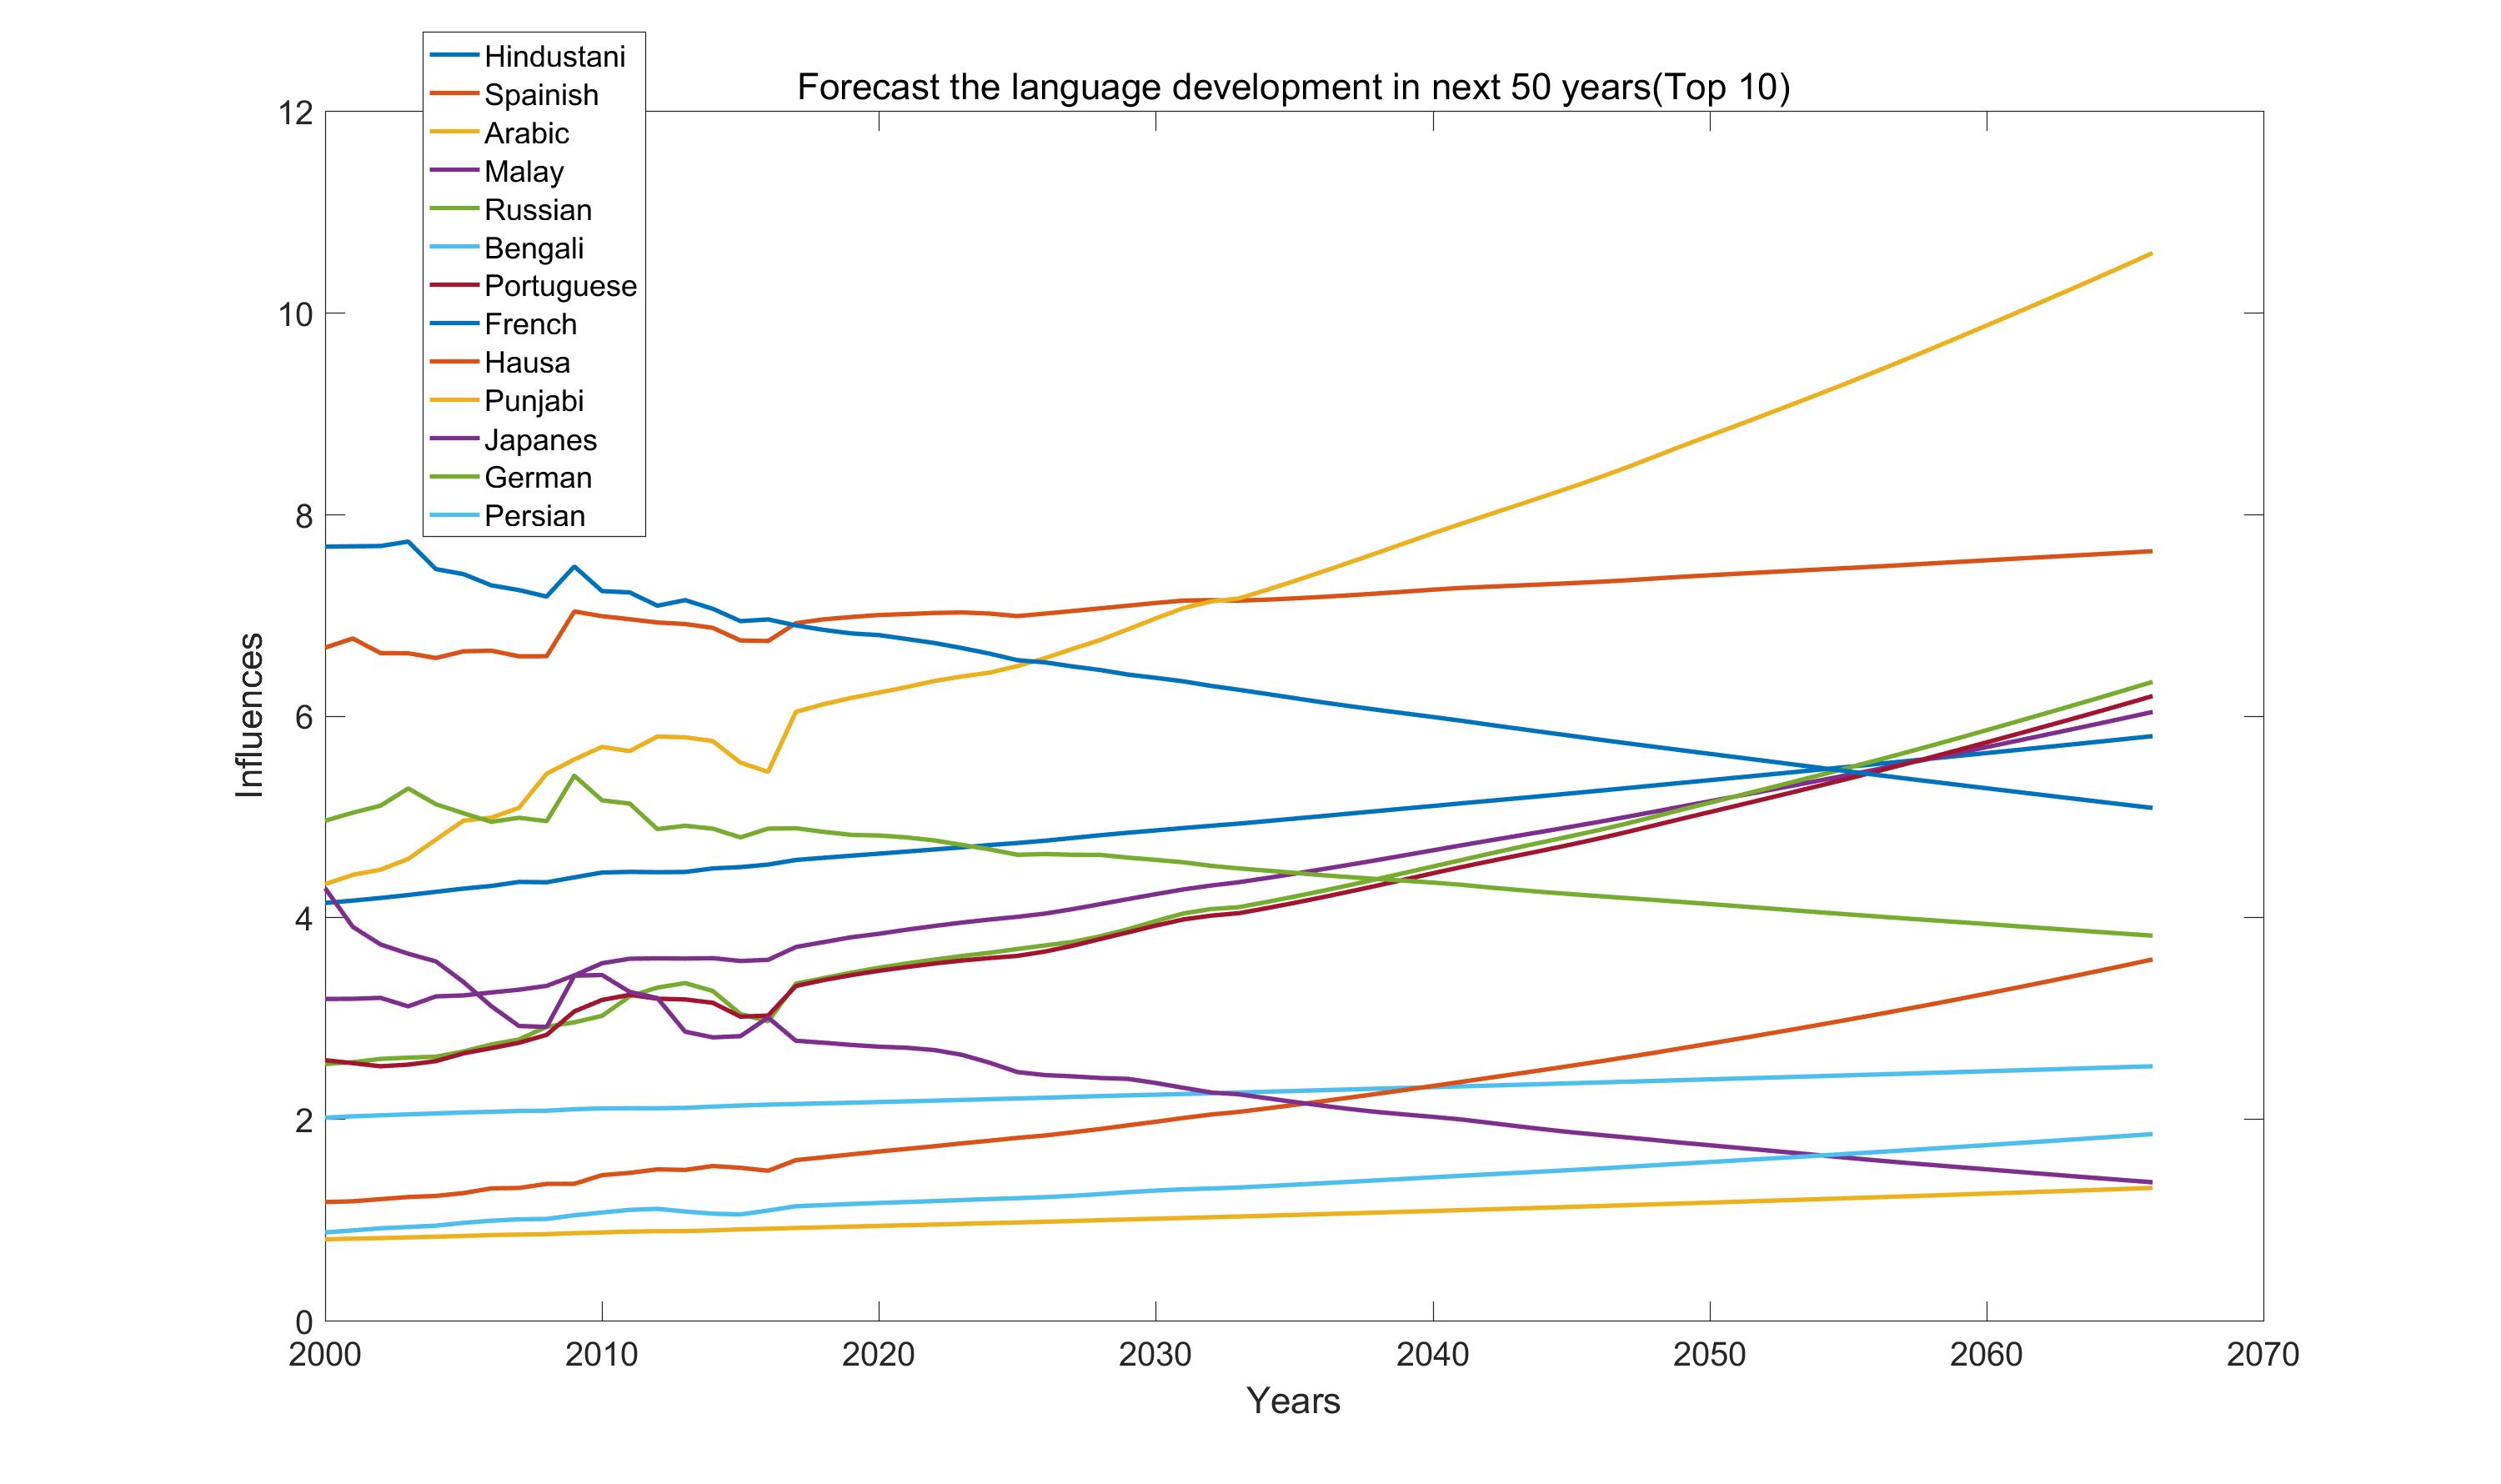
\includegraphics[width=7.5cm]{icf2.jpg}
\caption{Influences ranking prediction(ignore top 2)}
\end{minipage}
\end{figure}

Figure 1 and 2 show how the influence change in the next 50 years. Refer to the figure, Chinese and English would dominate the futher, 
and Chinese transcend English to become world common language in 2038. 

\section{Validating the Model}
\subsubsection{The influences of the model}
\qquad We use the contral variable method



After the calculation of the Fuzzy Synthetic Evaluation Model, we obtain the global distribution of all total different languages speakers. Then we established economic model to choose the place to open a office.
The model cosider the business effect and the profits that the company may receive.


\subsection{Growth of influences model}
\qquad We build up this model based on Fuzzy Synthetic Evaluation Model, growing number of
\begin{table}[h]
\begin{center}
{\hspace{-1in}
\begin{minipage}{\textwidth}
\fontsize{10}{12}\selectfont
\begin{tabular}[c]{lrrrrrr}
\toprule
              & \multicolumn{2}{c}{1900} & \multicolumn{2}{c}{1906} & \multicolumn{2}{c}{1910}\\
\cmidrule(r){2-3}\cmidrule(lr){4-5}\cmidrule(l){6-7}
Party         & \% of Vote  & Seats Won  & \% of Vote  & Seats Won  & \% of Vote  & Seats Won \\
\midrule
\addlinespace
              & \multicolumn{6}{c}{Provincial Assembly}\\
\cmidrule{2-7}
Conservative  & 35.6        &  47        & 26.0        & 37         & 30.9        & 52\\
Socialist     & 12.4        &  18        & 27.1        & 44         & 24.8        & 39\\
Christian Democrat & 49.2   &  85        & 41.2        & 68         & 39.2        & 59\\
Other         & 2.8         &  0         & 5.7         & 1          & 5.1         & 0\\
\addlinespace
Total& 100.0       &  150       & 100.0       & 150        & 100.0       & 150\\
\addlinespace
              & \multicolumn{6}{c}{National Assembly}\\
\cmidrule{1-7}
Conservative  & 32.6        &   4        & 23.8        &  3         & 28.3        & 3\\
Socialist     & 13.5        &   1        & 27.3        &  3         & 24.1        & 2\\
Christian Democrat & 52.0   &   7        & 42.8        &  6         & 46.4        & 8\\
Other         & 1.8         &   0        & 6.1         &  0         & 1.2         & 0\\
\addlinespace
Total& 100.0       &  12        & 100.0       & 12         & 100.0       & 13\\
\bottomrule
\end{tabular}
\end{minipage}
}
\caption[Elections in G\"{o}tefrith province, 1900--1910]{Elections in
  G\"{o}tefrith province, 1900--1910.  (Taken from \cite{chicago},
  pg.~414.)}%
\label{tab:chicago-table}
\end{center}
\end{table}

\section{Conclusions}



\section{Evaluate of the Model}

\section{Strengths and weaknesses}


\subsection{Strengths}
\begin{itemize}
\item \textbf{Applies widely}\\
This  system can be used for many types of airplanes, and it also
solves the interference during  the procedure of the boarding
airplane,as described above we can get to the  optimization
boarding time.We also know that all the service is automate.
\item \textbf{Improve the quality of the airport service}\\
Balancing the cost of the cost and the benefit, it will bring in
more convenient  for airport and passengers.It also saves many
human resources for the airline. \item \textbf{}
\end{itemize}
\cite{chicago}
\subsection{Weaknesses}
\begin{itemize}
\item \textbf{Policy never change}\\
The model works only depand on no any outside force disturb, for instance: Policy won't change, and 
wherever is stable.
\item \textbf{Data insufficient}\\

\end{itemize}
\newpage 
\section{Memo}
\begin{center}
\large {\textbf {MEMORANDUM}}
\end{center}
\textbf {To}: Chief Operating Officer \\
\textbf {From}: Team \#84802 \\
\textbf {Subject}: The best location to open office \\
\textbf {Date}: February 13,2018 \\
\noindent\rule[0.25\baselineskip]{\textwidth}{1pt}
\paragraph{} 

\bibliographystyle{plain}
\bibliography{mcm}

\begin{appendices}

\section{First appendix}


Here are simulation programmes we used in our model as follow.

\textbf{\textcolor[rgb]{0.98,0.00,0.00}{Input matlab source:}}
\lstinputlisting[language=Matlab]{./code/poly_forecast.m}

\section{Second appendix}

some more text \textcolor[rgb]{0.98,0.00,0.00}{\textbf{Input C++ source:}}
\lstinputlisting[language=C++]{./code/mcmthesis-sudoku.cpp}

\end{appendices}

\end{document}

